\documentclass[10pt,        % Don't change the font size!
               a4paper,     % Don't change the paper size!
               journal,     % Journal paper format
%               draft       % Enable this parameter to get a draft version.
               ]{IEEEtran}
\makeatletter


\def\markboth#1#2{\def\leftmark{\@IEEEcompsoconly{\sffamily}\MakeUppercase{\protect#1}}%
\def\rightmark{\@IEEEcompsoconly{\sffamily}\MakeUppercase{\protect#2}}}
\makeatother
%\usepackage[latin1]{inputenc}
\usepackage[utf8]{inputenc}

\usepackage[T1]{fontenc}
% If IEEEtran.cls has not been installed into the LaTeX system files,
% manually specify the path to it like:
% \documentclass[journal]{../sty/IEEEtran}

% *** GRAPHICS RELATED PACKAGES ***
%
\ifCLASSINFOpdf
  \usepackage[pdftex]{graphicx}
  % declare the path(s) where your graphic files are
  \graphicspath{{../pdf/}{../jpeg/}}
  % and their extensions so you won't have to specify these with every instance of \includegraphics
  \DeclareGraphicsExtensions{.pdf,.jpeg,.png}
\else
  % or other class option (dvipsone, dvipdf, if not using dvips). graphicx
  % will default to the driver specified in the system graphics.cfg if no driver is specified.
  % \usepackage[dvips]{graphicx}
  % declare the path(s) where your graphic files are
  % \graphicspath{{../eps/}}
  % and their extensions so you won't have to specify these with every instance of \includegraphics
  % \DeclareGraphicsExtensions{.eps}
\fi

% correct bad hyphenation here
\hyphenation{op-tical net-works semi-conduc-tor}

\begin{document}
\title{Relational and NoSQL Databases: A Comparison and Introduction to Hybrid and Mining Frameworks}

\author{Teodor Fratiloiu}% <-this % stops a space

% The paper headers
\markboth{Scientific Seminar on Security in Information Technology, Winter Semester 2020/2021}%
{Teodor Fratiloiu: Comparison of SQL Relational Databases and NoSQL Graph Databases}

\maketitle


\begin{abstract}
%\boldmath
Classic, relational, SQL databases have proven their reliability, and versatility, in many different scenarios over the past few decades. However wide their field of applications may be though, there are still many situations, where one can be limited by the constraints of these traditional data structures. Efficiently querying very large user databases is one such situation. In this work, we are going to investigate a different paradigm for  big data management: Graph Databases. This \textit{relatively} new breed of data management systems are already finding wide acceptance across many industries, and are being actively deployed. Use cases such as social media applications come to mind, where scalability is of prime importance - these datasets could theoretically grow to infinite dimensions, after all. In this work, we will compare Graph (NoSQL) databases, as well as their strengths, and weaknesses, to classic, relational, SQL databases. We will also dive into innovative new technologies, which promise to enable new ways of working with databases and making sense of the data inside.
\end{abstract}

\textbf{Keywords:} Relational SQL Database, Graph NoSQL Database, Tablespace, Graph Mining, Hybrid Database

\section{Introduction}
Databases have been used as the prime way of storing data in digital formats for the better part of the past 70 years since computer memory became large enough to enable this in the 1960s. It is safe to assume that virtually every kind of tabular data, which has since been digitalized, has been converted into one such database, or a closely related approximation thereof. \cite{bachman_1973} \par
The history of databases has often been divided into 3 separate phases: firstly, there was the \textit{classical} period of navigational databases (which strongly relied on the period's ever present memory pointers). This was followed by the invention of the relational (SQL) database by IBM's researchers in the early 1970s \cite{codd_1970}. Lastly, around the turn of the millennia, researchers came up with the modern, post-SQL (or NoSQL) database, which has the distinction of having \textit{no fixed structure}, or much in the way of theoretical constraints related to its overall architecture, if at all. \par
The reason for the existence of these new, very flexible types of databases has much to do with the main issue of classic, SQL databases. It is the exponential way in which hardware requirements scale up with the amount of data stored. This means that it becomes exponentially more challenging to maintain speed, RAM, and storage amounts within reasonable constraints as the amount of stored data increases. This problem of SQL databases has been steadily developing over the decades, and it has to do with the difficulties that arise when mixing legacy database rules with the realities of modern, distributed, and connected devices. \cite{IEEEpaper1:comparison} \par
Let us, therefore, introduce NoSQL databases. The main difference between these, and SQL databases, is how they scale. While SQL databases scale \textit{vertically}, NoSQL databases scale \textit{horizontally}. Specifically, it is the BASE (Basically Available State and Eventually Consistent) property of NoSQL databases which enables them to be a perfect choice for very large, connected, amounts of data. \par
For this paper, we shall consider the term \textit{relational} database (RDBMS) as synonymous to \textit{SQL} database, and the term \textit{NoSQL} database as equivalent to \textit{Graph} database, unless other specified. As such, the respective pairs of terms will be used interchangeably. \par
It has been proved in the research literature, as well as by the industry, that Graph databases perform radically better than relational databases for big data applications. \cite{IEEEpaper1:comparison} This is especially true in scenarios where one can use the connected nature of data to their advantage. One prominent example of this is how Neo4j (NoSQL) performs much better than Oracle 11g (SQL). \cite{comparison_2015} \par
However, let us not forget that Graph databases are not the only kind of NoSQL database. There are four types in total. Let us examine these in detail. 
\begin{itemize}
	\item \textbf{Key-Value}: these are, essentially, hash tables, where unique hash keys are used to search for and point to specific values; the contents themselves are not used for queries.
	\item \textbf{Document}: Data is stored as a key/value tuple, and both the content, as well as the \textit{key} are used for searches, which constitutes a major difference from the type above. Documents of this type can be stored in XML, JSON, and BSON formats, and popular apps using this type of database include MongoDB and CouchDB.
	\item \textbf{Wide-Column}: These databases are made unique by the hybrid approach used to store data. In this scenario, which is mainly used in \textit{cluster environments} and for distributed data, we will combine the features of relational databases with a key-value storage schema. Examples such as Hbase, Cassandra, and Accumulo spring to mind.
	\item \textbf{Graph}: This type is used where the data has a high degree of connectivity since such databases can naturally store relationships between Independent pieces of data. Examples include Neo4j, Pregel, ArrangoDB, and OrientDB. 
\end{itemize}
Actual examples, together with actual package names, query languages and properties, can be found in \textit{Table \ref{table_types_nosql}}. \cite{IEEEpaper1:comparison}

\begin{table}[!t]
	\renewcommand{\arraystretch}{1.3} % increase table row spacing, adjust to taste
	\caption{NoSQL Database Frameworks and Their Features}
	\label{table_types_nosql}
	\centering
	\begin{tabular}{|p{1.1cm}|p{1.2cm}|p{2.3cm}|p{2.3cm}|} 
		\hline
		Type & Package & Query Language & Transaction Support  \\
		\hline
		Graph & Neo4j & CypherQL & ACID \\
		\hline
		Graph & ArangoDB & AQL & ACID support for Multi-Document \\
		\hline
		Graph & OrientDB & SQL & ACID \\
		\hline
		Key-Value & Riak & Custom Subset of SQL &  Partial ACID Support (CID)\\
		\hline
		Key-Value & Redis & Custom Syntax & Partial ACID support (ACI)\\
		\hline
		Key-Value & Voldemort & Custom API & Partial ACID support \\
		\hline
		Column & Hbase & Custom API (Java) & Limited ACID\\
		\hline
		Column & Accumulo & Custom API (Java, Python, PHP, Ruby) & ACID \\
		\hline
		Document & MongoDB & Custom API & ACID \\
		\hline
		Document & CouchDB & Fauxton \cite{gh_couchdb} & ACID \\
		\hline
	\end{tabular}
\end{table}

Having delivered our remarks about the fundamental differences between SQL and Graph Databases, let us proceed with a more detailed description of the current state of of these databases in the industry, as well as investigating how wide their rollut and applications currently are.

\section{State of the Art}
In this section, we shall look into, and compare, the different properties of SQL and NoSQL databases. For starters, let us revisit the scalability issue. As previously discussed, the more varied and larger the amount of data present in a SQL database, the more CPU and RAM a system will need. This is because relational databases scale \textit{vertically}, in contrast to NoSQL databases, which scale \textit{horizontally}. \par
SQL databases are traditionally a good fit for applications where data integrity and security are important, since cryptographic procedures and information security can be more easily implemented in such a scenario. NoSQL databases, however, are a great fit for very large, and growing, datasets, because they allow us to, for instance, add extra storage servers to an existing system with minimal intervention. The following theoretical exercise might help one understand this better. \par
\subsection{The CAP Theorem}
To enable us to better understand the fundamental differences between relational and Graph databases, let us introduce Eric Brewer's \textit{CAP Theorem} - Consistency, Availability and Partition Tolerance. \cite{brewer_cap_theorem} A term by term analysis looks as follows: \textit{Consistency} describes the property of a system of achieving a \textit{stable state}, after one (or more) \textit{write} operations. \textit{Availability} describes data, namely, it being present and ready for \textit{read} operations at one desired spot, after having been modified (right there or somewhere else). \textit{Partition Tolerance} refers to a system's ability to continue functioning, even if its resources are spread over different locations and nodes. \par
In relational databases, primary keys are used to ensure that the data is \textit{unique} - it exists in one single location. NoSQL databases, on the other hand, and in no small part due to their distributed nature, cannot provide such a feature. But let us not believe that this would have to be a bad thing. NoSQL databases will, because of this, be much more flexible and responsive to the changes one would experience in a connected system, for instance. Moreover, tracking interaction between different objects is much easier in this scenario. \par
However, we shall quickly realize that there is one obvious \textit{catch} to all of this: a distributed database system can never offer true CAP features. Not in a logically rigorous manner, at least. That is because the intrinsic nature of how the data is stored in such a system cannot guarantee total and immediate consistency. Let us think about how data propagates across the internet. For the purpose of this, let one imagine they would change one's online profile picture for their Google profile, on their desktop. After the change is done, let one immeaditely pick up their smartphone and open the YouTube app, where they had already been logged in with their Google account. One can very sensibly assume that the picture the user would see on their smartphone, at least for the first few moments, will be their old profile picture. This goes to prove that, for a brief period of time, that one user had \textit{two different profile pictures}, at the same time. A state which very obviously contradicts any form of consistency. \par
To sum up, let one remember that relational databases traditionally possess all 3 CAP properties, whereas NoSQL databases (depending on the implementation) customarily only support the \textit{Availability} and \textit{Partition Tolerance} parts, but lack the \textit{Consistency} feature. Let us now look out over on the other side of the fence, and see how relational, SQL databases fare. \par
As such, let us now dive into the specific advantages and disadvantages afforded by the underlying technologies and the very nature of these two kinds of databases, respectively. 

\section{Methods and Contributions}
\subsection{On SQL and the Importance of Information Security}

As previously discussed, relational databases support the ACID (atomicity, consistency, isolation, and durability) property. This ensures that we can reliably implement data security-related measures for our data. For instance, Kumar et al. explain in \cite{nosql_db_sec} how financial applications need to provide guarantees that monetary amounts are accurate all the time, and that there is absolutely no doubt whatsoever about how much one's account is worth at a given time. Any such ambiguity would be unacceptable for a financial application, as it could potentially allow for tampering and abuse. As described by Brook et al. in \cite{brook_hf_trading}, let one imagine a very fast trading bot that would capitalize on such a loophole by performing \textit{two} identical purchase orders in \textit{very} fast succession, faster than the system could account for the cost of the first one, and therefore buy the second asset for virtually zero money since their total capital had remained unchanged since the first buy. \par
For this reason, we are limited to only using SQL databases for such sensitive applications as financial platforms. Using them requires us to separate and log our different actions utilizing \textit{orders} or \textit{transactions} - which ensures atomicity and isolation. Each of these transactions would then need to be centrally approved before changing any data in the actual database - therefore ensuring consistency and durability. Unfortunately, such guarantees would never be possible with a pure Graph database (one without modifications and extra provisions, that is). As such, let us look into how we could potentially get the benefits of both worlds, with a hybrid approach.\par

\subsection{The Hybrid Approach}
In their 2019 paper, Vyawahare and Karde \cite{IEEEpaper3:hybrid} make a comprehensive review of past scientific literature on the topic of hybrid databases. Let us explain their main points, as well as their contributions. \par
The main assumption the authors make about enabling a hybrid database approach is the fact that we need a minimum of 2 databases, of the same or different kinds, which we can access through a common \textit{abstraction layer}. In layman's terms, this implies that one would have to come up with a know-it-all software framework, capable of linking databases of all kinds, and enabling a coherent mix-match of data types of all shapes and sizes, which would ideally work together. \par
The workflow proposed in the paper is relatively straightforward. One would start by loading and analyzing data, determining whether its structure would be a better fit for either the relational or the NoSQL sides of the harmonized, hybrid database, then store that data appropriately. Obviously, there are many variations that can be made to these steps. For example, one could use the hybrid framework to simply convert databases of one type into the other, to benefit from the advantages of the other side. One could also use the framework to harmonize the types of queries used in their apps and reduce the overhead generated by having to use multiple querying languages. Finally, the authors go into some detail about the advantages of keeping data \textit{in memory}. These mostly revolve around access times, and availability, plus reducing the storage and processing overhead generated by real-time data conversion. \par
Having now seen the hybrid approach to database design, let us look into how we can make sense of the data inside our databases by what is known as \textit{Graph Mining Framework}, as described in \cite{IEEEpaper2:mining}.

\subsection{Data Mining and NoSQL Graph Visualization}
In the day and age of the internet, where data is being generated and saved at \textit{breakneck} speed, making sense of this content has become a matter of automated analysis. Conveniently, one very important application of NoSQL (Graph) Databases is their enabling more robust, and faster, data mining. \par
The main features a NoSQL \textit{graph mining} tool would have to provide include graph preprocessing, association discovery, cluster detection, and graph visualization. Let us investigate these in detail. \par
Firstly, graph preprocessing is to be understood as an \textit{umbrella} term for all the necessary steps to transform data from an arbitrary format, such as \textit{XML} or the result of web-crawling, into a specific format for our application. The data would be stored as an undirected graph, with non-unique labeled edges. \cite{IEEEpaper2:mining} Secondly, when it comes to association discovery, we could set arbitrary thresholds for the number of edges connecting different nodes and the types of nodes we are looking at. This would allow us to, for example, discover popular actor-director pairs in a movie database. Third, if we were to detect data clusters, we could, for instance, use algorithms such as trawling \cite{paper_2_ref_1}, shingling \cite{paper_2_ref_2}, connection subgraphs \cite{paper_2_ref_3}, or maximum clique detection \cite{paper_2_ref_4}, which would enable our framework to answer questions such as identifying one user's social media friends, or the number of news articles on one particular topic. Lastly, a form of graph visualization would allow one to input data in some arbitrary text-based descriptive format and receive a visual representation of this graph. \par
One such framework would enable data scientists to make more sense of the plethora of data available in the highly-distributed and large NoSQL databases of today's internet. 

\section{Results} 
For this section, we will compare the access (read and write) performance of different types of databases. 
\subsection{Numerical Comparisons}
For this subsection, let us observe some plots. In \textit{Figure \ref{graph_phys_vs_neo4j}}, we can see how a physically optimized relational database fares against a graph database. \textit{Figure \ref{graph_no_phys_vs_neo4j}} shows us the longer access times when there is no physical optimization. The actual numerical times are presented in \textit{Figure \ref{table_phys_vs_neo4j}}, and \textit{Figure \ref{table_no_phys_vs_neo4j}}, respectively. \par
\begin{figure}[!t]
	\centering
	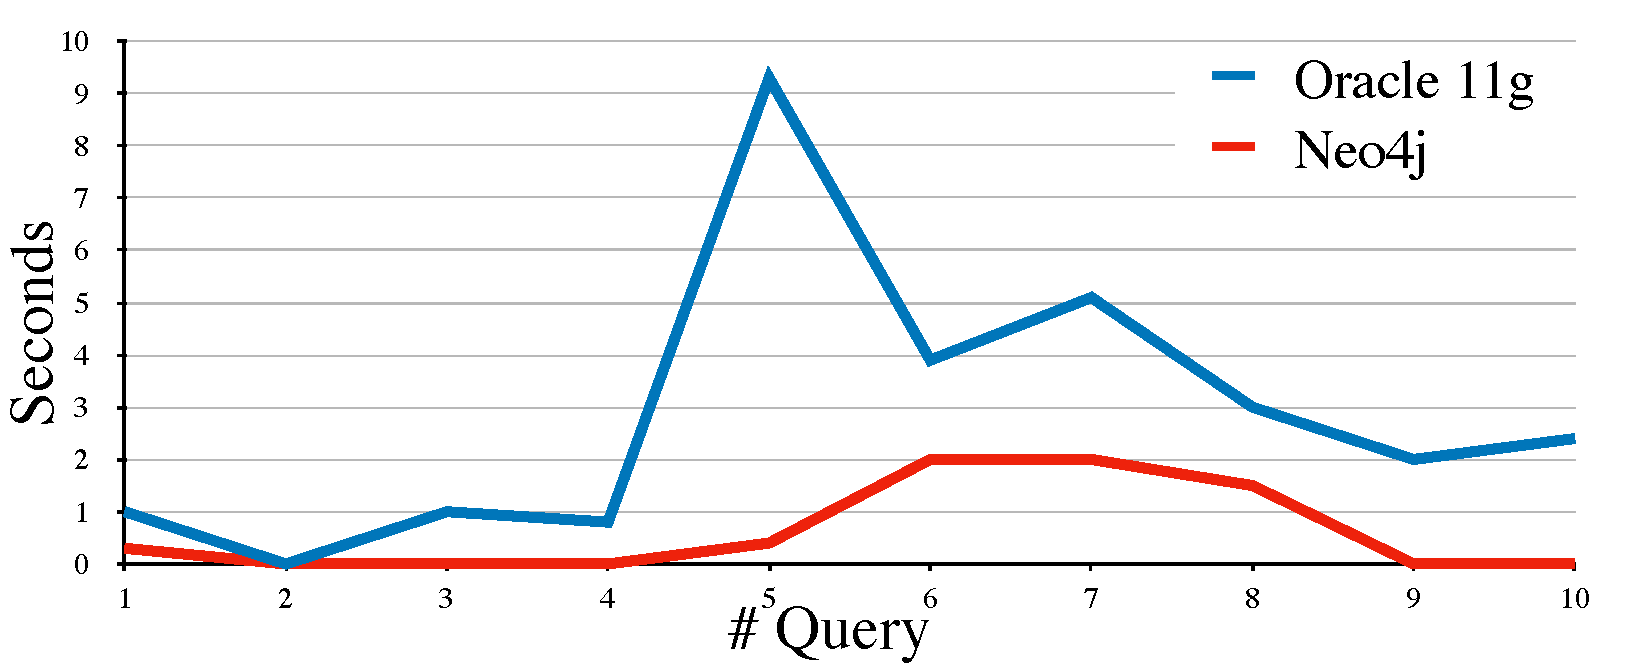
\includegraphics[width=2.5in]{plots/phys_vs_neo4j}
	\caption{Performance Comparison of Neo4j with a tuned RDB \cite{IEEEpaper1:comparison}}
	\label{graph_phys_vs_neo4j}
\end{figure}

\begin{figure}[!t]
	\centering
	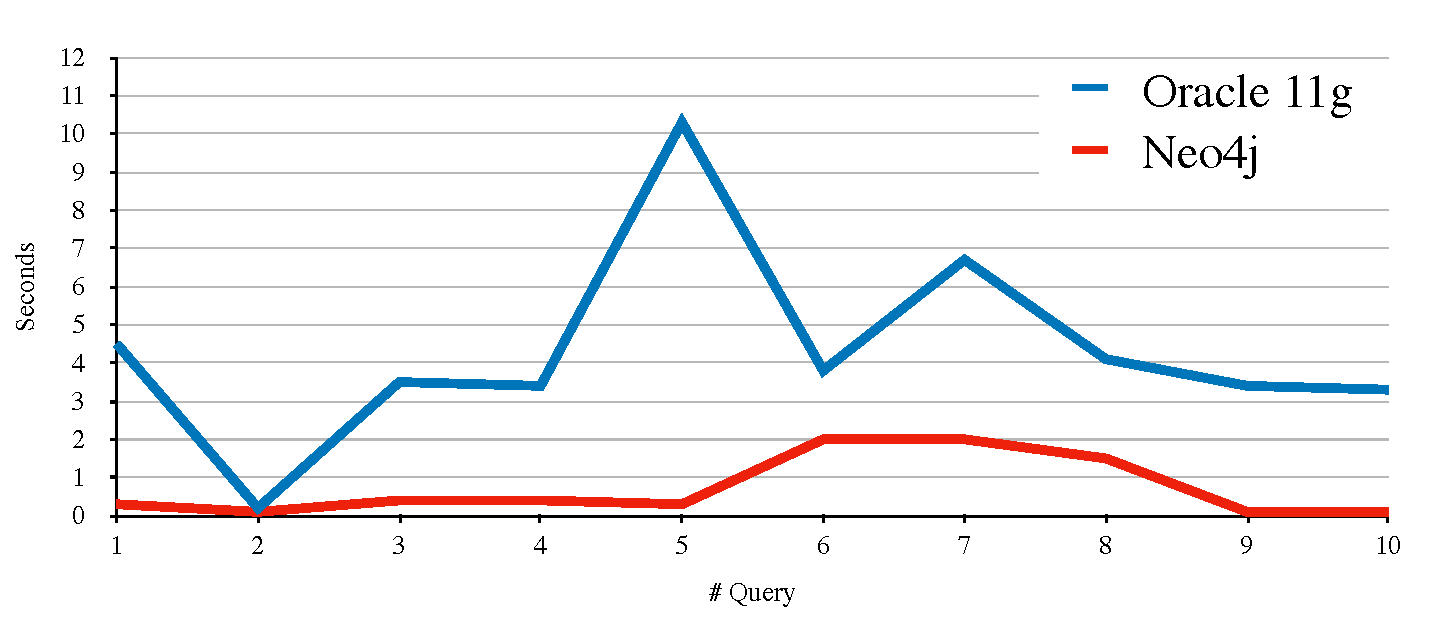
\includegraphics[width=2.5in]{plots/no phys vs neo4j}
	\caption{Performance Comparison of Neo4j with a non-tuned RDBS \cite{IEEEpaper1:comparison}}
	% \vspace{-0.7cm}
	\label{graph_no_phys_vs_neo4j}
\end{figure}


\begin{figure}[!t]
	\centering
	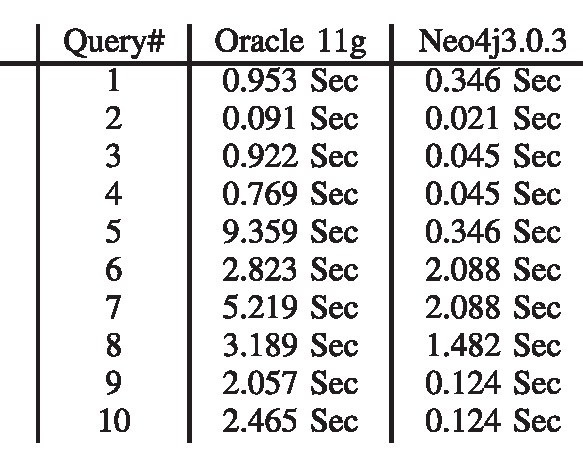
\includegraphics[width=2.8in]{plots/phys vs neo4j table}
	\caption{Performance Comparison of (physically optimized) Oracle 11g with Neo4j, according to Khan et al. \cite{IEEEpaper1:comparison}}
	\label{table_phys_vs_neo4j}
\end{figure}

\begin{figure}[!t]
	\centering
	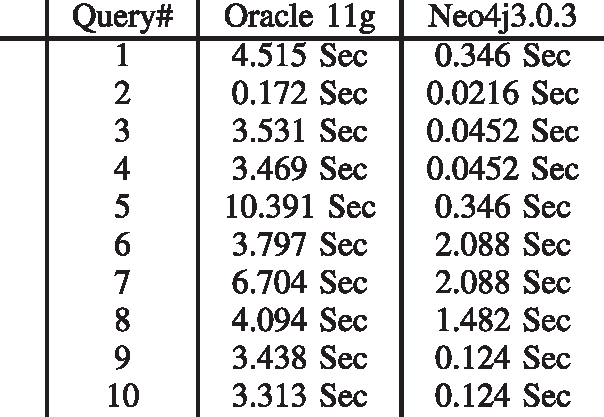
\includegraphics[width=2.8in]{plots/no tuning table}
	\caption{Performance Comparison of Oracle 11g (no physical optimization) with Neo4j, according to Khan et al. \cite
	{IEEEpaper1:comparison}}
	\label{table_no_phys_vs_neo4j}
\end{figure}


\subsection{Relational Database Design Optimization}
In this subsection, we shall examine the results and performance achieved by tuning relational databases, why this is so important, and why one should always consider doing it, both when deploying a product, and when running benchmarks on standard data to determine speed. \par
Let us look into how the performance of classic databases can be optimized. To this end, a process called \textit{tuning} can be involved. For instance, to improve the query performance of \textit{Oracle 11g} tables, we can use different tablespaces for each individual schema.  This results in more than one data file used for storage, which in turn allows us to optimize the size of the memory blocks used. This is useful, since both small and large memory block sizes can be desirable, depending on the scenario. For example, \textit{warehouse-type} data requires large memory blocks, whereas, for \textit{OLTP} type data, we are required to use small block sizes. The total space allocation in a file is defined as an \textit{extent}, whereas one unit of I/O data is referred to as a \textit{block}. 
The ACID (Atomicity, Consistency Isolation, Durability) property of SQL databases helps maintain consistency across the data and enables efficient polling and querying, but even this is eventually overcome by the sheer size of modern databases for online, user-generated content. \par
Even if SQL databases store data in separate tables, and normalization techniques, such as 1NF, 2NF, and 3NF, can be used to reduce redundancy, this method remains unsuitable for modern applications. For instance, although it is possible to \textit{join} queries when searching a SQL database for entries, this too becomes inefficient when using 20 or more parameters. \par
Judging by this, and by the thoughts expressed in the previous subsection, we can conclude that both sides prove to have specific design limitations, which are impossible to directly overcome. \par
\subsection{Main Take-Aways}
Firstly, it is widely accepted that NoSQL, Graph databases are the desirable way to store data  when systems are distributed and when flexibility, and redundancy, are needed. Such fields as online shops, social media, or some remote working tools rely on this type of system architecture, to ensure responsiveness and reliable operation for multi-user collaboration. Further development and standardization of such systems could potentially open the doors to increased efficiency and reduced costs across the industry. \par
On the other hand, relational databases still play a very important role in centralized, high-value, or mission-critical data. It is only with this type of database that one can ensure the reliable storage of such information like medical records, employment and financial histories, or voter registrations. Future research in this area could involve the development of even more sophisticated file systems, optimized for fast flash storage, or increasing information security by means of tightening standards for advanced encryption and by rolling out more and more granular access control. \par 
Moreover, let us once more stress the fact that we do not assert the superiority of either database type over the other. We remain strongly convinced that both have their own strengths and weaknesses, which one only needs to be aware of when making the choice about which best suits their needs. It is exactly for this reason that we presented the Hybrid approach to database design, in which many see an acceptable compromise. \par

\section{Conclusion}
Having now accomplished what we set out to do - namely to present a thorough analysis, and comparison, of the two most common types of databases in use throughout industries in this day and age, let us now deliver the closing remarks and express our hope that have at least awoken the community's interest for further research on the topic. 

\begin{thebibliography}{3}

\bibitem{IEEEpaper1:comparison}
W. Khan, W. Ahmad, B. Luo and E. Ahmed, SQL Database with Physical Tuning Technique and NoSQL Graph Database Comparisons (2019)

\bibitem{IEEEpaper2:mining}
Swapnil Shrivastava and Supriya N. Pal, Graph Mining Frameworks for Finding and Visualizing Substructures using Graph Databases (2009)

\bibitem{IEEEpaper3:hybrid}
H.R. Vyawahare, P.P. Karde and V.M. Thakare, A Hybrid Database Approach Using Graph and Relational Database (2019)

\bibitem{bachman_1973}
Bachman, Charles W., The Programmer as Navigator (1973)

\bibitem{codd_1970}
E. Codd, A Relational Model of Data for Large Shared Data Banks (1970)

\bibitem{comparison_2015}
Oussous, A., F.-Z. Benjelloun, A. A. Lahcen, and S. Belfkih, Comparison and Classication of NoSQL Databases for Big Data (2015)

\bibitem{brewer_cap_theorem}
S. Gilbert and N. Lynch, "Brewer's conjecture and the feasibility of consistent, available, partition-tolerant web services"

\bibitem{paper_2_ref_1}
R. Kumar, P. Rafhavan, S. Rajagopalan, A. Tomkins, "Thrawling the Web for Emerging Cybercommunities" (1999)

\bibitem{paper_2_ref_2}
D. Gibson, R. Kumar, A. Tomkins, "Extracting Large, Dense Subgraphs in Massive Graphs" (2005)

\bibitem{paper_2_ref_3}
C. Faloutsos, K. McCurley, A. Tomkins, "Fast Discovery of Connection Subgraphs" (2004)

\bibitem{paper_2_ref_4}
I.M. Bomze, M. Budinich, P.M. Pardalos, M. Pelillo, "The Maximum Clique Problem" (1999)

\bibitem{gh_couchdb}
Apache CouchDB GitHub Repository - https://github.com/apache/couchdb-fauxton (Retrieved 01/17/2021)

\bibitem{nosql_db_sec}
J. Kumar and V. Garg, "Security analysis of unstructured data in NOSQL MongoDB database," (2017)

\bibitem{brook_hf_trading}
M. Brook, C. Sharp, G. Ushaw, W. Blewitt and G. Morgan, "Volatility Management of High Frequency Trading Environments," (2013)

\end{thebibliography}

\end{document}


